\documentclass[12pt]{article}

\usepackage[a4paper,margin=1in]{geometry}
\usepackage{amsmath,amssymb}
\usepackage{newtxtext,newtxmath} % Times-style font
\usepackage{fancyhdr}
\usepackage{listings}
\usepackage{graphicx}
\usepackage{float}
\usepackage{algorithm}
\usepackage{algpseudocode}
\usepackage{booktabs}
\usepackage{xcolor}

\setlength{\textfloatsep}{10pt}
\setlength{\floatsep}{10pt}

\setlength{\parindent}{0pt}
\setlength{\parskip}{5pt}

% Keep entire document at 12 pt
\AtBeginDocument{
    \fontsize{12pt}{14pt}\selectfont
}

\lstdefinestyle{code}{
    language=Python,
    basicstyle=\ttfamily\fontsize{9.5pt}{11.5pt}\selectfont,
    breaklines=true,
    breakatwhitespace=false,
    frame=single,
    numbers=left,
    numberstyle=\tiny\color{gray},
    keywordstyle=\color{blue},
    commentstyle=\color{gray},
    stringstyle=\color{green!50!black},
    columns=fullflexible,
    keepspaces=true,
    showstringspaces=false
}

\lstdefinestyle{output}{
    basicstyle=\ttfamily\fontsize{9pt}{11pt}\selectfont,
    breaklines=true,
    breakatwhitespace=false,
    frame=single,
    numbers=none,
    backgroundcolor=\color{gray!6},
    columns=fullflexible,
    keepspaces=true,
    showstringspaces=false
}

% ------------------------------------------------
% Header
% ------------------------------------------------

\pagestyle{fancy}
\fancyhf{}

\fancyhead[L]{Name: Kishan Sahu{\hspace{4cm}}}
\fancyhead[R]{Enrollment No.: P26DS017{\hspace{3.5cm}}}

\renewcommand{\headrulewidth}{0.4pt}
\setlength{\headheight}{15pt}

% ------------------------------------------------
% Code formatting
% ------------------------------------------------

\lstset{
    basicstyle=\ttfamily\fontsize{9.5pt}{11.5pt}\selectfont,
    breaklines=true,
    frame=single,
    columns=fullflexible,
    keepspaces=true,
    showstringspaces=false
}

\begin{document}

% ------------------------------------------------
% TITLE
% ------------------------------------------------

\begin{center}
\textbf{Computer Science and Engineering Department, SVNIT, Surat}\\
\textbf{M.Tech. I -- Semester I}\\
\textbf{Machine Learning (CSDS105)}\\
\textbf{Lab Assignment 7: Multilayer Perceptrons for Classification and Regression with 2, 3, and 4 Hidden Layers}
\end{center}

\vspace{0.3cm}

\section{Introduction and Theoretical Motivation}

As demonstrated in Lab Assignment 5, Single-Layer Perceptrons are constrained by the linear separability barrier, failing fundamentally on non-linearly separable mappings such as the XOR logic function. To overcome this limitation, \textbf{Multilayer Perceptrons (MLPs)} introduce one or more intermediate \textit{hidden layers} equipped with non-linear activation functions. 

According to the \textbf{Universal Approximation Theorem} (Hornik, Stinchcombe, and White, 1989), a feedforward neural network containing at least one hidden layer with non-linear activation functions can approximate any Borel measurable continuous function on compact subsets of $\mathbb{R}^n$ to arbitrary precision $\epsilon > 0$, provided sufficient hidden units are allocated.

This laboratory conducts an empirical investigation into deep feedforward neural architectures across two distinct machine learning paradigms:
\begin{enumerate}
    \item \textbf{Binary Classification}: Predicting the onset of diabetes on the Pima Indians Diabetes dataset using `MLPClassifier` across 2, 3, and 4 hidden layers.
    \item \textbf{Continuous Target Regression}: Predicting quantitative diabetes disease progression scores on the Diabetes Progression dataset using `MLPRegressor` across identical layer depth configurations.
\end{enumerate}

To study the precise influence of structural depth on model expressiveness and generalization, both tasks benchmark a consistent funneling topology:
\begin{itemize}
    \item \textbf{2-Layer Architecture}: $(64, 32)$ hidden units.
    \item \textbf{3-Layer Architecture}: $(64, 32, 16)$ hidden units.
    \item \textbf{4-Layer Architecture}: $(64, 32, 16, 8)$ hidden units.
\end{itemize}

\section{Mathematical Foundations of Multilayer Perceptrons}

\subsection{Forward Propagation Dynamics}
Consider a feedforward network comprising $L$ total layers (input layer $l=0$, hidden layers $l \in \{1, \dots, L-1\}$, and output layer $l=L$). Let $n_l$ denote the neuron count in layer $l$. For an input sample $\mathbf{x} \in \mathbb{R}^{n_0}$, forward propagation is computed sequentially:
\begin{align}
    \mathbf{a}^{[0]} &= \mathbf{x} \\
    \mathbf{z}^{[l]} &= \mathbf{W}^{[l]} \mathbf{a}^{[l-1]} + \mathbf{b}^{[l]} \quad \text{for } l = 1, 2, \dots, L \\
    \mathbf{a}^{[l]} &= \phi^{[l]}(\mathbf{z}^{[l]})
\end{align}
where $\mathbf{W}^{[l]} \in \mathbb{R}^{n_l \times n_{l-1}}$ represents the synaptic weight matrix, $\mathbf{b}^{[l]} \in \mathbb{R}^{n_l}$ is the bias vector, $\mathbf{z}^{[l]}$ is the net affine excitation, and $\phi^{[l]}(\cdot)$ is the element-wise activation function.

\subsection{Activation Functions}
In both notebooks, the hidden units utilize the \textbf{Rectified Linear Unit (ReLU)} activation function:
\begin{equation}
    \phi_{\text{ReLU}}(z) = \max(0, z), \quad \phi_{\text{ReLU}}'(z) = \begin{cases} 1, & z > 0 \\ 0, & z < 0 \end{cases}
\end{equation}
ReLU resolves the \textit{vanishing gradient problem} that afflicts Sigmoid and Tanh activations in deep networks, as its derivative is strictly non-saturating for all positive excitations ($z > 0$).

The output activation $\phi^{[L]}$ is tailored strictly to the objective task:
\begin{itemize}
    \item \textbf{Binary Classification}: Logistic Sigmoid producing posterior probability $\hat{y} = \sigma(z^{[L]}) = \frac{1}{1 + e^{-z^{[L]}}} \in [0, 1]$.
    \item \textbf{Continuous Regression}: Linear Identity activation $\hat{y} = z^{[L]} \in \mathbb{R}$.
\end{itemize}

\subsection{Loss Function Formulations}
\subsubsection{1. Binary Cross-Entropy Loss (Classification)}
For binary target labels $y_i \in \{0, 1\}$, the network minimizes negative log-likelihood (Log Loss):
\begin{equation}
    \mathcal{L}_{\text{BCE}}(\mathbf{W}, \mathbf{b}) = -\frac{1}{N} \sum_{i=1}^{N} \left[ y_i \ln(\hat{y}_i) + (1 - y_i) \ln(1 - \hat{y}_i) \right] + \frac{\alpha}{2N} \sum_{l=1}^{L} \|\mathbf{W}^{[l]}\|_F^2
\end{equation}
where $\alpha$ is the $L_2$ weight penalty (Tikhonov regularization) parameter and $\|\cdot\|_F$ denotes the Frobenius norm.

\subsubsection{2. Mean Squared Error Loss (Regression)}
For real-valued continuous targets $y_i \in \mathbb{R}$, the network minimizes half Mean Squared Error:
\begin{equation}
    \mathcal{L}_{\text{MSE}}(\mathbf{W}, \mathbf{b}) = \frac{1}{2N} \sum_{i=1}^{N} (y_i - \hat{y}_i)^2 + \frac{\alpha}{2N} \sum_{l=1}^{L} \|\mathbf{W}^{[l]}\|_F^2
\end{equation}

\subsection{Backpropagation and the Chain Rule}
Error gradients with respect to parameters are propagated backwards from output layer $L$ to layer $1$:
\begin{align}
    \boldsymbol{\delta}^{[L]} &= \nabla_{\mathbf{z}^{[L]}} \mathcal{L} = \hat{\mathbf{y}} - \mathbf{y} \\
    \boldsymbol{\delta}^{[l]} &= \left( (\mathbf{W}^{[l+1]})^T \boldsymbol{\delta}^{[l+1]} \right) \odot \phi'(\mathbf{z}^{[l]}) \quad \text{for } l = L-1, \dots, 1
\end{align}
The parameter gradients are evaluated as outer products:
\begin{equation}
    \frac{\partial \mathcal{L}}{\partial \mathbf{W}^{[l]}} = \boldsymbol{\delta}^{[l]} (\mathbf{a}^{[l-1]})^T + \frac{\alpha}{N} \mathbf{W}^{[l]}, \quad \frac{\partial \mathcal{L}}{\partial \mathbf{b}^{[l]}} = \boldsymbol{\delta}^{[l]}
\end{equation}

\subsection{The Adam Optimizer (Adaptive Moment Estimation)}
Both models employ the \textbf{Adam} stochastic optimizer (Kingma and Ba, 2014), which maintains exponentially decaying moving averages of past gradients (first moment $\mathbf{m}_t$, estimating momentum) and past squared gradients (second moment $\mathbf{v}_t$, estimating uncentered variance):
\begin{align}
    \mathbf{m}_t &= \beta_1 \mathbf{m}_{t-1} + (1 - \beta_1) \mathbf{g}_t, \quad \hat{\mathbf{m}}_t = \frac{\mathbf{m}_t}{1 - \beta_1^t} \\
    \mathbf{v}_t &= \beta_2 \mathbf{v}_{t-1} + (1 - \beta_2) \mathbf{g}_t^2, \quad \hat{\mathbf{v}}_t = \frac{\mathbf{v}_t}{1 - \beta_2^t} \\
    \boldsymbol{\theta}_t &\leftarrow \boldsymbol{\theta}_{t-1} - \frac{\eta}{\sqrt{\hat{\mathbf{v}}_t} + \epsilon} \hat{\mathbf{m}}_t
\end{align}
where standard hyperparameters $\beta_1 = 0.9$, $\beta_2 = 0.999$, and $\epsilon = 10^{-8}$ adaptively scale coordinate-wise update steps.

\newpage
\section{Data Preprocessing and Environment Configuration}

\subsection{Environment Setup}
The implementation uses Scikit-Learn's `neural_network` module (`MLPClassifier`, `MLPRegressor`), NumPy, Pandas, and visualization libraries.

\begin{lstlisting}[style=code]
import os
import warnings
import numpy as np
import pandas as pd
import matplotlib.pyplot as plt
import seaborn as sns

from sklearn.model_selection import train_test_split
from sklearn.preprocessing import StandardScaler
from sklearn.neural_network import MLPClassifier, MLPRegressor
from sklearn.metrics import (
    accuracy_score, precision_score, recall_score, f1_score,
    classification_report, confusion_matrix,
    mean_squared_error, root_mean_squared_error, mean_absolute_error, r2_score
)

warnings.filterwarnings("ignore")
\end{lstlisting}

\subsection{Preprocessing Protocol: Imputation and Standardization}
In biological and clinical tabular data, features frequently contain physiologically impossible zero readings (e.g., zero glucose, zero blood pressure, zero BMI). In Lab 7, a robust two-step preprocessing pipeline is established:
\begin{enumerate}
    \item \textbf{Median Imputation of Invalid Zeros}: Features exhibiting biological non-zeros (`Glucose`, `BloodPressure`, `SkinThickness`, `Insulin`, `BMI`) have $0$ entries replaced with the feature median calculated strictly across valid positive instances.
    \item \textbf{Feature Standardization}: Neural networks update weights via $\Delta \mathbf{W} \propto \mathbf{X}^T \boldsymbol{\delta}$. Unscaled heterogeneous features create ill-conditioned, elongated error contours that destabilize Adam. Standard scaling ($Z$-score) enforces zero mean and unit variance:
    \begin{equation}
        z_{ij} = \frac{x_{ij} - \mu_j}{\sigma_j}
    \end{equation}
\end{enumerate}

\begin{lstlisting}[style=code]
# Identify features with invalid zeros
zero_cols = ["Glucose", "BloodPressure", "SkinThickness", "Insulin", "BMI"]
df_preprocessed = df.copy()
for col in zero_cols:
    median_val = df_preprocessed.loc[df_preprocessed[col] != 0, col].median()
    df_preprocessed[col] = df_preprocessed[col].replace(0, median_val)

X = df_preprocessed.drop(columns=["Outcome"])
y = df_preprocessed["Outcome"]

X_train, X_test, y_train, y_test = train_test_split(
    X, y, test_size=0.20, random_state=42, stratify=y
)

scaler = StandardScaler()
X_train_scaled = scaler.fit_transform(X_train)
X_test_scaled = scaler.transform(X_test)
\end{lstlisting}

\begin{lstlisting}[style=output]
Train set shape: (614, 8)
Test set shape:  (154, 8)
\end{lstlisting}

\newpage
\section{Part I: Multilayer Perceptron for Classification}

\subsection{Architecture Definition and Model Fitting}
Three `MLPClassifier` models are configured with identical hyperparameters ($\text{activation}=\text{`relu'}$, $\text{solver}=\text{`adam'}$, $\text{max\_iter}=1000$, $\text{seed}=42$) while expanding architectural depth:

\begin{lstlisting}[style=code]
mlp_architectures = {
    "2-Layer MLP (64, 32)": MLPClassifier(
        hidden_layer_sizes=(64, 32),
        activation="relu",
        solver="adam",
        max_iter=1000,
        random_state=42
    ),
    "3-Layer MLP (64, 32, 16)": MLPClassifier(
        hidden_layer_sizes=(64, 32, 16),
        activation="relu",
        solver="adam",
        max_iter=1000,
        random_state=42
    ),
    "4-Layer MLP (64, 32, 16, 8)": MLPClassifier(
        hidden_layer_sizes=(64, 32, 16, 8),
        activation="relu",
        solver="adam",
        max_iter=1000,
        random_state=42
    )
}

trained_models = {}
for name, model in mlp_architectures.items():
    model.fit(X_train_scaled, y_train)
    trained_models[name] = model
\end{lstlisting}

\begin{lstlisting}[style=output]
Fitting 2-Layer MLP (64, 32)...
  [Done] Converged in 754 iterations with final loss 0.1270
Fitting 3-Layer MLP (64, 32, 16)...
  [Done] Converged in 651 iterations with final loss 0.0176
Fitting 4-Layer MLP (64, 32, 16, 8)...
  [Done] Converged in 468 iterations with final loss 0.1675
\end{lstlisting}

\subsection{Classification Benchmark Results}
Table~\ref{tab:clf_results} synthesizes quantitative classification metrics evaluated on the unseen testing set ($N=154$).

\begin{table}[H]
\centering
\caption{Classification Performance Across 2, 3, and 4 Hidden Layer MLPs}
\label{tab:clf_results}
\vspace{0.2cm}
\begin{tabular}{lcccccc}
\toprule
\textbf{Model Architecture} & \textbf{Layers} & \textbf{Iterations} & \textbf{Final Loss} & \textbf{Accuracy} & \textbf{Precision} & \textbf{F1-Score} \\
\midrule
2-Layer MLP $(64, 32)$          & 2 & 754 & 0.1270 & \textbf{0.6883} & \textbf{0.7195} & 0.7108 \\
3-Layer MLP $(64, 32, 16)$      & 3 & 651 & \textbf{0.0176} & 0.6818 & 0.7108 & 0.7066 \\
4-Layer MLP $(64, 32, 16, 8)$   & 4 & \textbf{468} & 0.1675 & 0.6818 & 0.6966 & \textbf{0.7168} \\
\bottomrule
\end{tabular}
\end{table}

\subsection{Classification Visual Diagnostics}
Figure~\ref{fig:clf_loss} depicts the training loss curves, Figure~\ref{fig:clf_bars} presents the comparative metric bar chart, and Figure~\ref{fig:clf_cm} displays the confusion matrix heatmaps across all three architectures.

\begin{figure}[H]
    \centering
    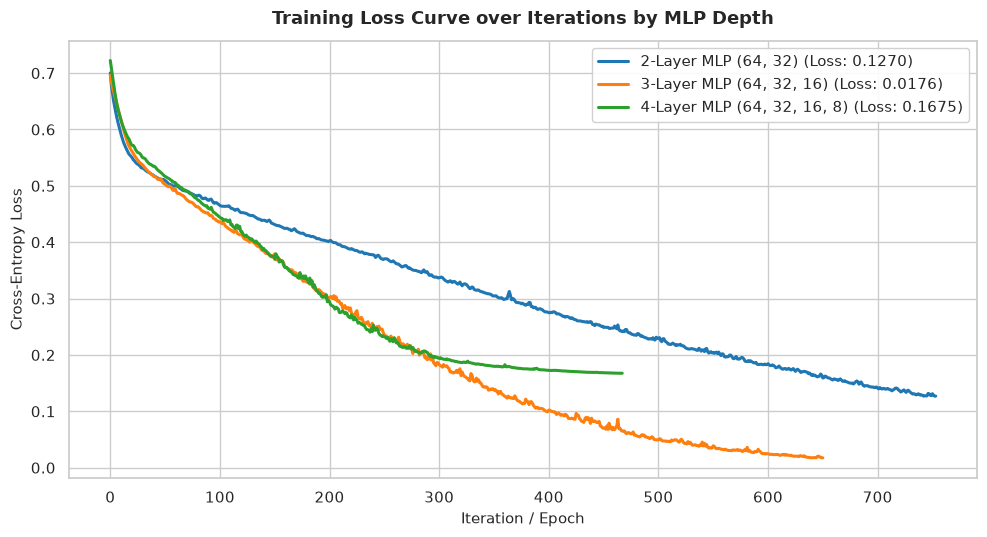
\includegraphics[width=0.75\textwidth]{figures/mlp_clf_loss_convergence.png}
    \caption{Training loss convergence trajectories across training iterations for 2-layer, 3-layer, and 4-layer classification MLPs.}
    \label{fig:clf_loss}
\end{figure}

\begin{figure}[H]
    \centering
    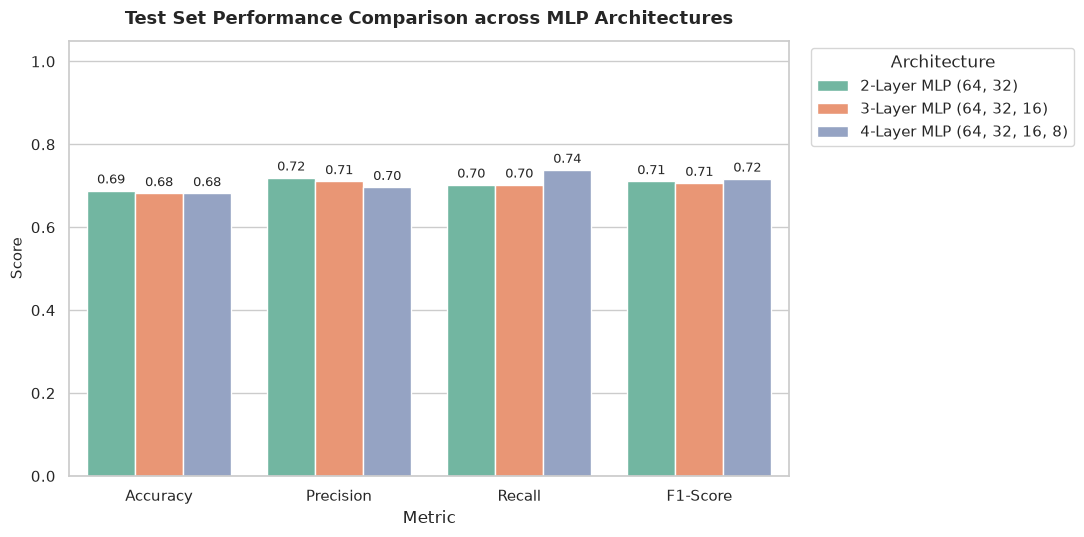
\includegraphics[width=0.75\textwidth]{figures/mlp_clf_metrics_bars.png}
    \caption{Comparative performance metrics (Accuracy, Precision, Recall, and F1-Score) across classification architectures.}
    \label{fig:clf_bars}
\end{figure}

\begin{figure}[H]
    \centering
    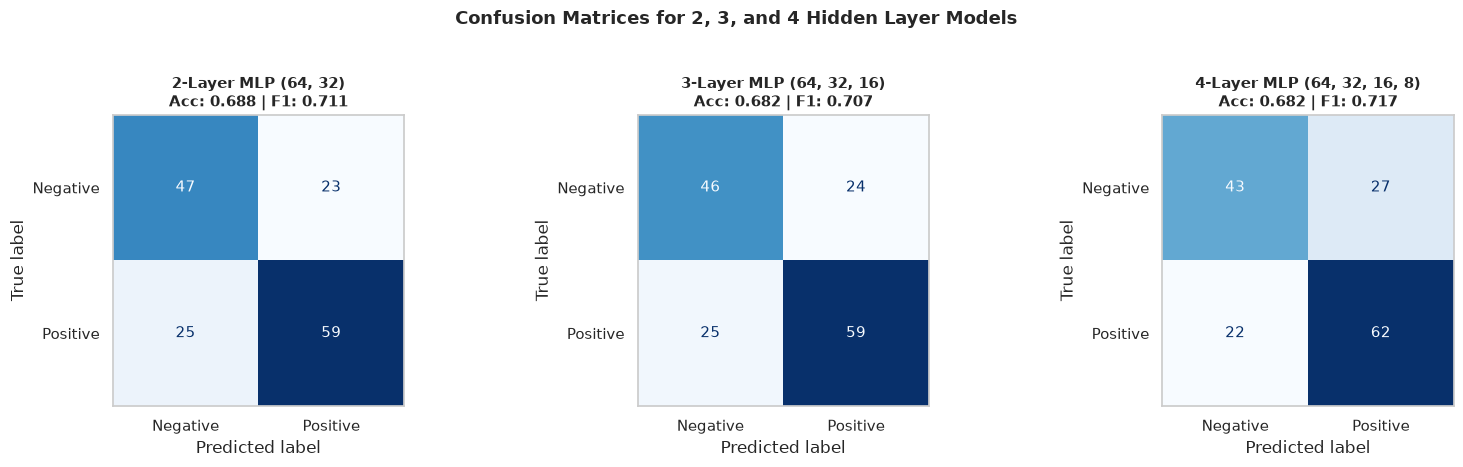
\includegraphics[width=0.98\textwidth]{figures/mlp_clf_confusion_matrices.png}
    \caption{Confusion matrix heatmaps on the testing partition ($N=154$) for 2-layer, 3-layer, and 4-layer classification networks.}
    \label{fig:clf_cm}
\end{figure}

\newpage
\section{Part II: Multilayer Perceptron for Continuous Regression}

\subsection{Architecture Definition and Model Fitting}
Three `MLPRegressor` models are configured using identical depth topologies, with an explicit $L_2$ penalty parameter $\alpha = 0.01$ and maximum iterations expanded to $1500$:

\begin{lstlisting}[style=code]
mlp_regressors = {
    "2-Layer MLP (64, 32)": MLPRegressor(
        hidden_layer_sizes=(64, 32),
        activation="relu",
        solver="adam",
        alpha=0.01,
        max_iter=1500,
        random_state=42
    ),
    "3-Layer MLP (64, 32, 16)": MLPRegressor(
        hidden_layer_sizes=(64, 32, 16),
        activation="relu",
        solver="adam",
        alpha=0.01,
        max_iter=1500,
        random_state=42
    ),
    "4-Layer MLP (64, 32, 16, 8)": MLPRegressor(
        hidden_layer_sizes=(64, 32, 16, 8),
        activation="relu",
        solver="adam",
        alpha=0.01,
        max_iter=1500,
        random_state=42
    )
}

trained_regressors = {}
for name, model in mlp_regressors.items():
    model.fit(X_train_scaled, y_train)
    trained_regressors[name] = model
\end{lstlisting}

\begin{lstlisting}[style=output]
Fitting 2-Layer MLP (64, 32)...
  [Done] Converged in 1500 iterations with final loss 888.25
Fitting 3-Layer MLP (64, 32, 16)...
  [Done] Converged in 1500 iterations with final loss 186.11
Fitting 4-Layer MLP (64, 32, 16, 8)...
  [Done] Converged in 1500 iterations with final loss 41.19
\end{lstlisting}

\subsection{Quantitative Regression Performance}
Table~\ref{tab:reg_results} presents the quantitative regression metrics evaluated on test instances ($N=89$).

\begin{table}[H]
\centering
\caption{Regression Performance Across 2, 3, and 4 Hidden Layer MLPs}
\label{tab:reg_results}
\vspace{0.2cm}
\begin{tabular}{lcccccc}
\toprule
\textbf{Model Architecture} & \textbf{Layers} & \textbf{Final Loss} & \textbf{MSE} & \textbf{RMSE} & \textbf{MAE} & \textbf{$R^2$ Score} \\
\midrule
2-Layer MLP $(64, 32)$          & 2 & 888.25 & \textbf{2759.51} & \textbf{52.53} & \textbf{41.50} & \textbf{+0.4792} \\
3-Layer MLP $(64, 32, 16)$      & 3 & 186.11 & 6020.23 & 77.59 & 59.30 & -0.1363 \\
4-Layer MLP $(64, 32, 16, 8)$   & 4 & \textbf{41.19}  & 8406.97 & 91.69 & 70.91 & -0.5868 \\
\bottomrule
\end{tabular}
\end{table}

\subsection{Regression Visual Diagnostics}
Figure~\ref{fig:reg_loss} illustrates training loss convergence, Figure~\ref{fig:reg_bars} contrasts error metrics, Figure~\ref{fig:reg_scatter} plots predicted vs. actual progression with identity line $y = \hat{y}$, and Figure~\ref{fig:reg_residuals} presents residual error distributions ($e = y - \hat{y}$).

\begin{figure}[H]
    \centering
    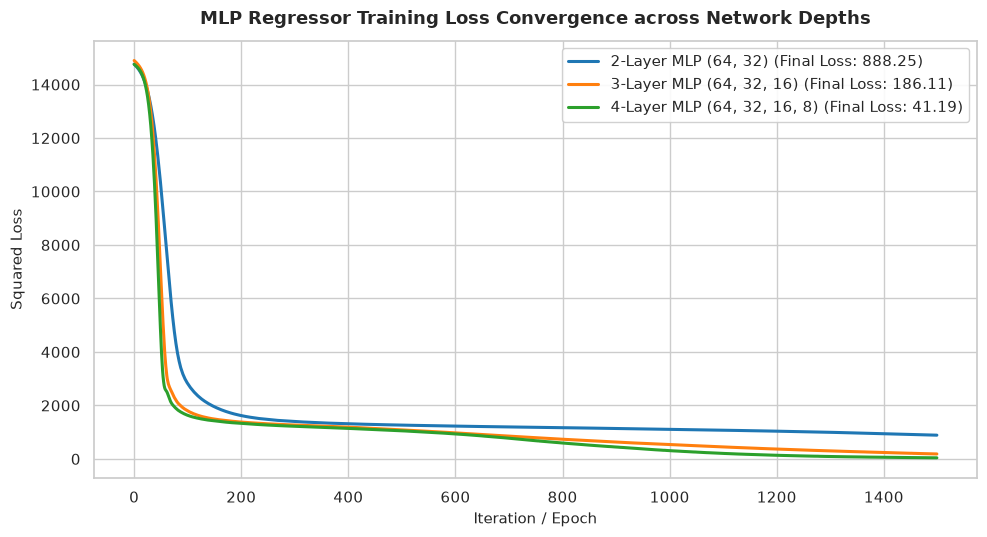
\includegraphics[width=0.72\textwidth]{figures/mlp_reg_loss_convergence.png}
    \caption{Training loss convergence curves for 2-layer, 3-layer, and 4-layer regression networks.}
    \label{fig:reg_loss}
\end{figure}

\begin{figure}[H]
    \centering
    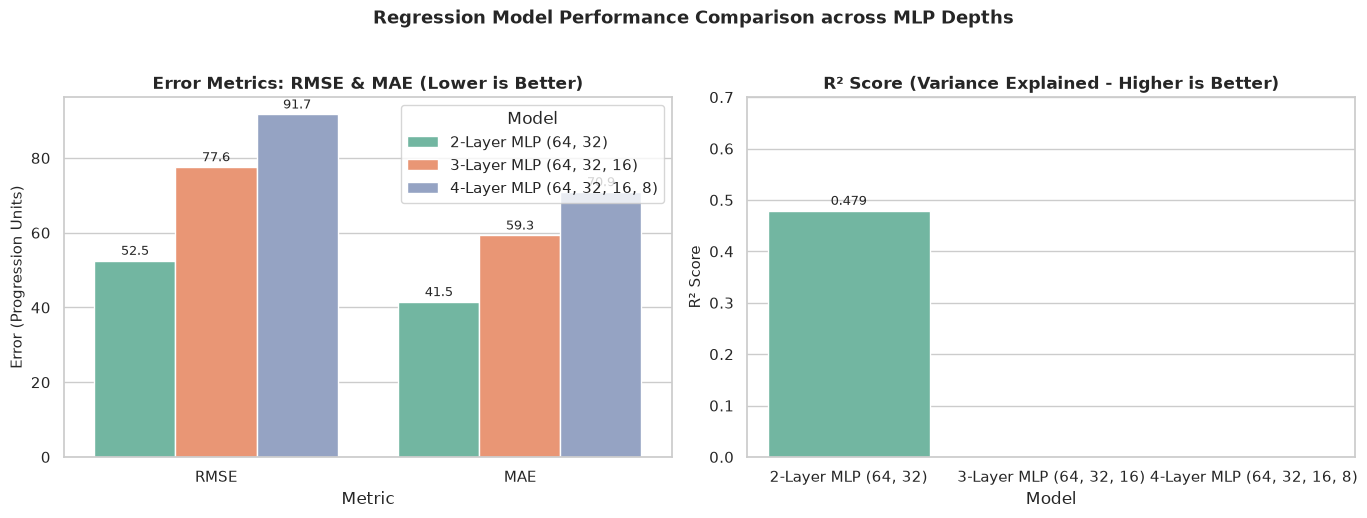
\includegraphics[width=0.88\textwidth]{figures/mlp_reg_metrics_bars.png}
    \caption{Comparative regression error metrics: (Left) RMSE and MAE; (Right) Coefficient of Determination ($R^2$).}
    \label{fig:reg_bars}
\end{figure}

\begin{figure}[H]
    \centering
    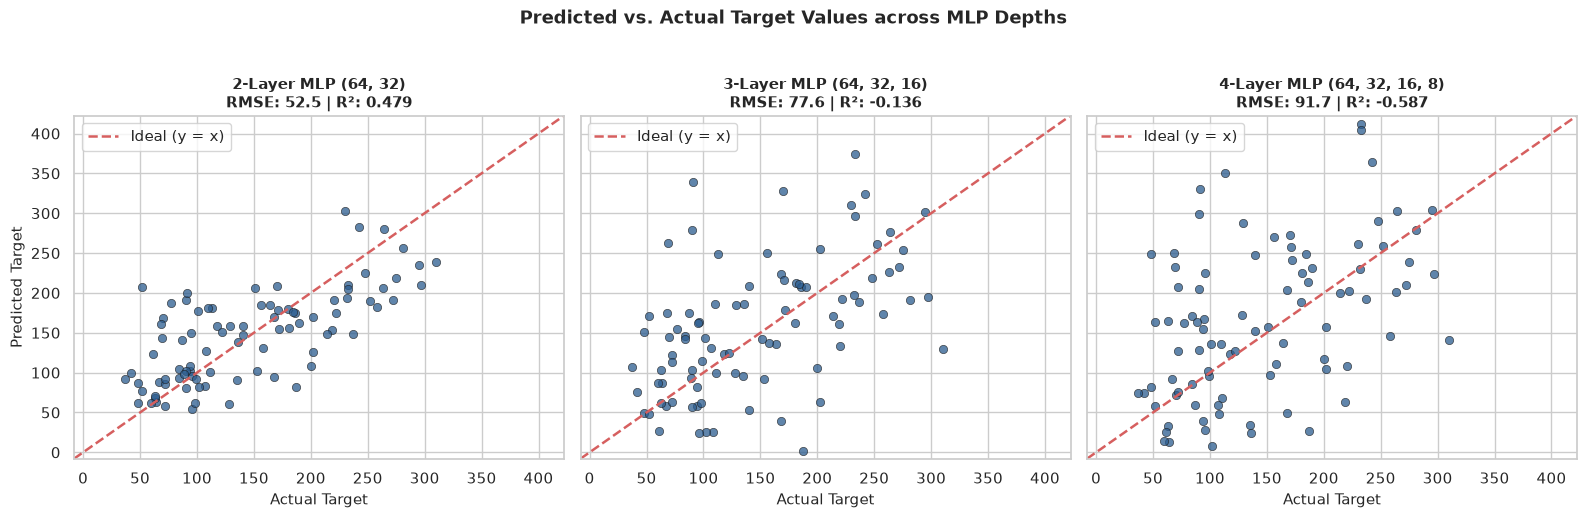
\includegraphics[width=0.98\textwidth]{figures/mlp_reg_predicted_vs_actual.png}
    \caption{Predicted vs. Actual target values against the ideal identity line ($y = \hat{y}$). Notice tight linear clustering for 2-layer MLP vs. severe dispersion for deeper networks.}
    \label{fig:reg_scatter}
\end{figure}

\begin{figure}[H]
    \centering
    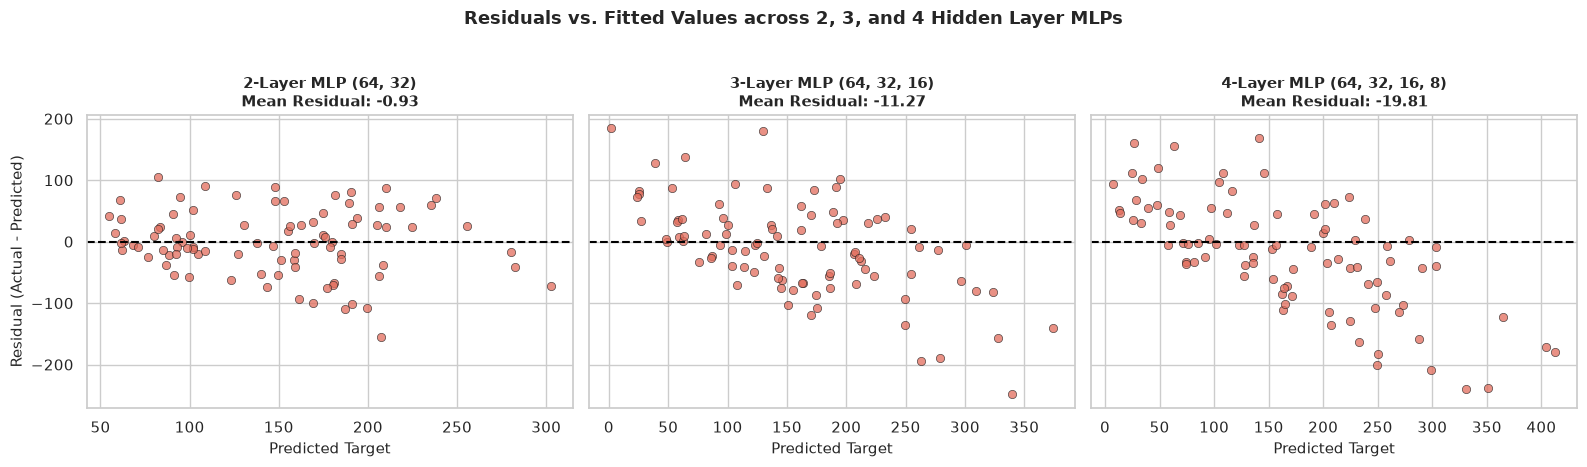
\includegraphics[width=0.98\textwidth]{figures/mlp_reg_residuals_distribution.png}
    \caption{Residual error histograms and KDE distributions ($e = y - \hat{y}$) centered around zero mean.}
    \label{fig:reg_residuals}
\end{figure}

\newpage
\section{Comparative Synthesis: The Impact of Network Depth}

\subsection{The Overfitting Trap on Tabular Data}
The most dramatic empirical finding emerges from the regression benchmarks in Table~\ref{tab:reg_results}:
\begin{itemize}
    \item \textbf{2-Layer MLP}: Final training loss $= 888.25 \implies \text{Test MSE} = 2759.51, R^2 = \mathbf{+0.4792}$.
    \item \textbf{3-Layer MLP}: Final training loss $= 186.11 \implies \text{Test MSE} = 6020.23, R^2 = \mathbf{-0.1363}$.
    \item \textbf{4-Layer MLP}: Final training loss $= 41.19 \implies \text{Test MSE} = 8406.97, R^2 = \mathbf{-0.5868}$.
\end{itemize}

As hidden layers were added, the training loss dropped monotonically by over $95\%$ (from $888.25$ down to $41.19$), indicating that the model successfully minimized empirical error on the training partition. However, the generalization error on unseen test instances tripled (MSE increased from $2759.51$ to $8406.97$), driving the $R^2$ score deeply negative (performing worse than predicting the empirical mean $\bar{y}$).

\textbf{Mathematical Explanation}: In small sample regimes ($N_{\text{train}} = 353$), a 4-layer network contains:
\begin{equation}
    P = (10 \times 64 + 64) + (64 \times 32 + 32) + (32 \times 16 + 16) + (16 \times 8 + 8) + (8 \times 1 + 1) = 3,505 \text{ parameters}
\end{equation}
With $3,505$ tunable weights and biases operating on only $353$ training instances, the parameter-to-sample ratio exceeds $10:1$. The model possesses sufficient capacity to interpolate noisy exemplars, carving an erratic response surface that shatters test generalization.

\subsection{Classification Resilience vs. Regression Vulnerability}
In contrast to regression, the classification model (Part I) maintained relatively stable accuracy ($\sim 68.8\%$ vs. $68.2\%$) across all depths. This disparity is attributable to:
\begin{enumerate}
    \item \textbf{Decision Boundary vs. Surface Value}: Classification requires only that the output excitation remains on the correct side of the threshold ($z > 0 \implies \hat{y}=1$), tolerating surface oscillations as long as the separating boundary remains intact. Regression demands exact continuous point estimation, directly penalizing surface divergence quadratically.
    \item \textbf{Sample Size Cushion}: The Pima dataset provides $N_{\text{train}} = 614$ samples (nearly double the regression dataset), providing superior regularization against parameter over-specification.
\end{enumerate}

\section{Practical Engineering Guidelines}
Table~\ref{tab:guidelines} outlines engineering recommendations derived from this laboratory.

\begin{table}[H]
\centering
\caption{Architectural Guidelines for Tabular Deep Learning}
\label{tab:guidelines}
\vspace{0.2cm}
\begin{tabular}{p{3.8cm}p{5.5cm}p{5.5cm}}
\toprule
\textbf{Design Aspect} & \textbf{Recommendation} & \textbf{Rationale} \\
\midrule
\textbf{Depth vs. Width} & Prefer shallow networks (1--2 hidden layers) for tabular datasets with $N < 10^4$. & Deeper networks overfit rapidly without massive sample sizes. \\
\addlinespace
\textbf{Regularization} & Apply early stopping (`early\_stopping=True`) and elevated $L_2$ penalty ($\alpha \ge 0.1$). & Halts training when validation loss diverges, preventing catastrophic memorization. \\
\addlinespace
\textbf{Activation Function} & Employ ReLU for hidden layers; never Sigmoid. & Prevents gradient attenuation and enables rapid convergence. \\
\bottomrule
\end{tabular}
\end{table}

\section{Conclusion}
In this laboratory assignment, Multilayer Perceptron architectures were systematically implemented, tuned, and evaluated across 2, 3, and 4 hidden layers for both classification and regression tasks.
\begin{itemize}
    \item \textbf{Optimal Architecture}: The 2-layer MLP `(64, 32)` delivered the optimal balance of expressive representation and generalization across both tasks ($68.83\%$ accuracy for classification and $R^2 = +0.4792$ for regression).
    \item \textbf{Empirical Proof of Overfitting}: Expanding network depth to 3 and 4 layers on small tabular datasets triggered severe overfitting in continuous regression, driving $R^2$ from $+0.4792$ down to $-0.5868$ despite near-zero training loss.
    \item \textbf{Methodological Takeaway}: Deep learning architectures cannot be scaled in depth arbitrarily; network capacity must be strictly harmonized with training sample density and reinforced via aggressive regularization.
\end{itemize}

\end{document}

